\begin{frame}{\insertsubsection}

  \begin{figure}[h]
    \center%
    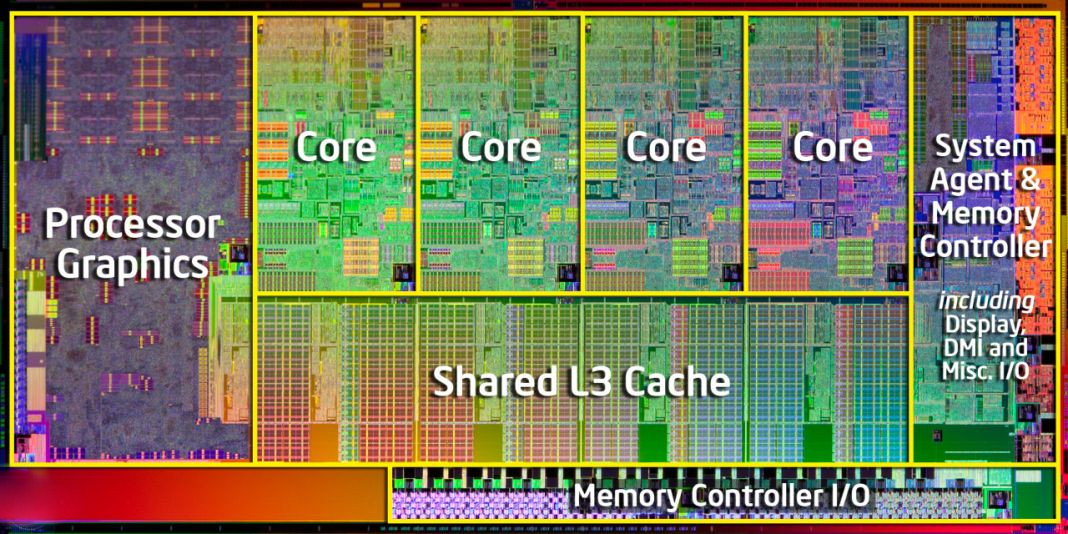
\includegraphics[height = .8\textheight]{multicore_cpu}
    \caption{Архитектура многоядерного процессора}
  \end{figure}

  \note{

    Современные процессоры состоят из множества крупных элементов:
    \textbf{ядер}, \textbf{графического процессора}, \textbf{общего кэша},
    \textbf{контроллера памяти} и других.

  }
\end{frame}

\begin{frame}<1-2>[label = core_elements]{\insertsubsection}

  \begin{figure}[h]
    \center%
    \begin{tikzpicture}[
      align = center,
      ->,
      > = Stealth,
      thick,
      mmu_node/.style = {
        rectangle,
        draw = Black,
        fill = ForestGreen,
        text = White,
      },
      cpu_node/.style = {
        rectangle,
        fill = PineGreen,
        draw = Black,
        text = White,
      },
      mem_node/.style = {
        rectangle,
        fill = Blue,
        draw = Black,
        text = White,
      },
      ]

      \node[mmu_node] (cr3) {
        CR3
      };

      \node[below = .5 of cr3,
      mmu_node,
      ] (pt_walker) {
        PT Walker
      };

      \node[left = of pt_walker,
      mmu_node,
      ] (tlb) {
        TLB
      };

      \node[
      inner sep = 8,
      fit = (tlb) (pt_walker) (cr3),
      draw = Black,
      label = above left:MMU,
      ] (mmu) {};

      \node[
      cpu_node,
      left = 2cm of mmu,
      yshift = 20,
      ] (exec_unit)  {
        Execution Unit
      };

      \node[
      cpu_node,
      below = of exec_unit,
      ] (load_unit) {
        Load/Store Unit
      };

      \node[mem_node,
      below = .6 of mmu,
      ] (l1_data) {
        L1 Data
      };

      \node[
      inner sep = 15,
      fit = (mmu) (load_unit) (exec_unit) (l1_data),
      draw = Black,
      label = above left:Ядро,
      ] (core) {};

      \node[mem_node, below = .2 of core] (l3) {
        L3 (Shared)
      };

      \node[mem_node, above = .75 of l3] (l2) {
        L2
      };

      \node<2>[
      fit = (exec_unit) (load_unit),
      line width = 0.5mm,
      draw = red,
      ] (fit_exec) {};

      \node<3>[
      fit = (l1_data) (l2) (l3),
      line width = 0.5mm,
      draw = red,
      ] (fit_cache) {};

      \node<4>[
      fit = (tlb) (pt_walker) (cr3),
      line width = 0.5mm,
      draw = red,
      ] (fit_mmu) {};

      \path (cr3)                edge                                       (pt_walker)
            (pt_walker.175)      edge node[above] {Fill}                    (tlb.10)
            (tlb.350)            edge node[below] {Miss}                    (pt_walker.185)
            (exec_unit.east)     edge[<->] node[below = .3cm] {Вирт. адрес} (mmu)
            (load_unit.east)     edge[<->]                                  (mmu)
            (mmu)                edge node[right] {Физ. адрес}              (l1_data)
            (l1_data)            edge                                       (l2)
            (l2)                 edge[<->]                                  (l3);

    \end{tikzpicture}
    \caption{Абстрактная архитектура элементов ядра, работающих с
      данными}\label{fig:core_elements}
  \end{figure}

  \note<1>{

    На рисунке \ref{fig:core_elements} представлен общий \textbf{план работы
      ядра с памятью и кэшем} в Intel процессорах. Более подробно об алгоритмах
    работы будет рассказано ниже.

    Современные процессоры представляют из себя \textbf{сильно
      распараллеливанные машины}, которые оперируют данными на высоких
    скоростях. Размеры процессоров уменьшаются, уменьшается потребление памяти
    используемое для вычисления одной и той же операции, что позволяет
    \textbf{увеличивать тактовую частоту}. Однако, существуют и другие способы
    уменьшить время, затрачиваемое на выполнение инструкций ---
    \textbf{различные оптимизации}, типы которых зависят от данных и состояния
    процессора.

    Рассмотрим некоторые \textbf{системы оптимизации, применяемые в ядрах и
      процессоре}.

  }

  \note<2->{

    Ниже \textbf{будет рассказано} о работе этих элементов.

  }
\end{frame}

\subsubsection{Конвейеризация}
\begin{frame}{\insertsubsubsection. По порядку}

  \begin{figure}[h]
    \begin{tikzpicture}[
      draw,
      align = center,
      ->,
      > = Stealth,
      thick,
      node distance = .6,
      block/.style = {
        rectangle,
        draw,
        fill = ForestGreen,
        text = White,
        text centered,
      },
      ]

      \node[block] (l1_i) {
        L1 I\$
      };

      \node[block, below = of l1_i] (if) {
        Instruction Fetch
      };

      \node[block, below = of if] (id) {
        Instruction Decode
      };

      \node[block, below = of id] (ie) {
        Instruction Execute
      };

      \node[block, below = of ie] (mem_acc) {
        Memory Access
      };

      \node[block, below = of mem_acc] (write) {
        Writeback
      };

      \node[block, left = of if] (bp) {
        Branch \\
        Predictor
      };

      \node[block, left = of mem_acc] (rf) {
        Register \\
        File
      };

      \node[block, right = 1.5 of mem_acc] (l1_d) {
        L1 \\
        D\$
      };

      \path (l1_i)    edge      (if)
            (if)      edge      (id)
            (id)      edge      (ie)
            (ie)      edge      (mem_acc)
            (mem_acc) edge      (write)
            (if)      edge      (bp)
            (l1_d)    edge[<->] (mem_acc);

      \draw (rf.north)   |- node{} (ie.west);
      \draw (write.west) -| node{} (rf.south);
      \draw (bp.south)   |- node{} (id.west);

    \end{tikzpicture}
    \caption{Элементы системы выполнения современного процессора (выполнение по
      порядку)}\label{fig:exe_in_order}
  \end{figure}

  \note{

    Конвейеризация --- одна из главных причин высокой скорости работы
    процессора. В результате данного процесса \textbf{работа с инструкциями
      разделяется} на несколько этапов (рисунок \ref{fig:exe_in_order},
    \textbf{выполнение инструкций по порядку}):

    \begin{itemize}
    \item \textbf{этап получения}, в результате которого код операции инструкции
      загружается в процессор;

    \item \textbf{этап декодирования}, в результате которого опкод декодируется
      во внутреннее представление процессора;

    \item \textbf{этап выполнения} --- инструкция исполняется.
    \end{itemize}

  }
\end{frame}

% \begin{frame}{\insertsubsubsection. Не по порядку}
%   \begin{figure}[h]
%     \center%
%     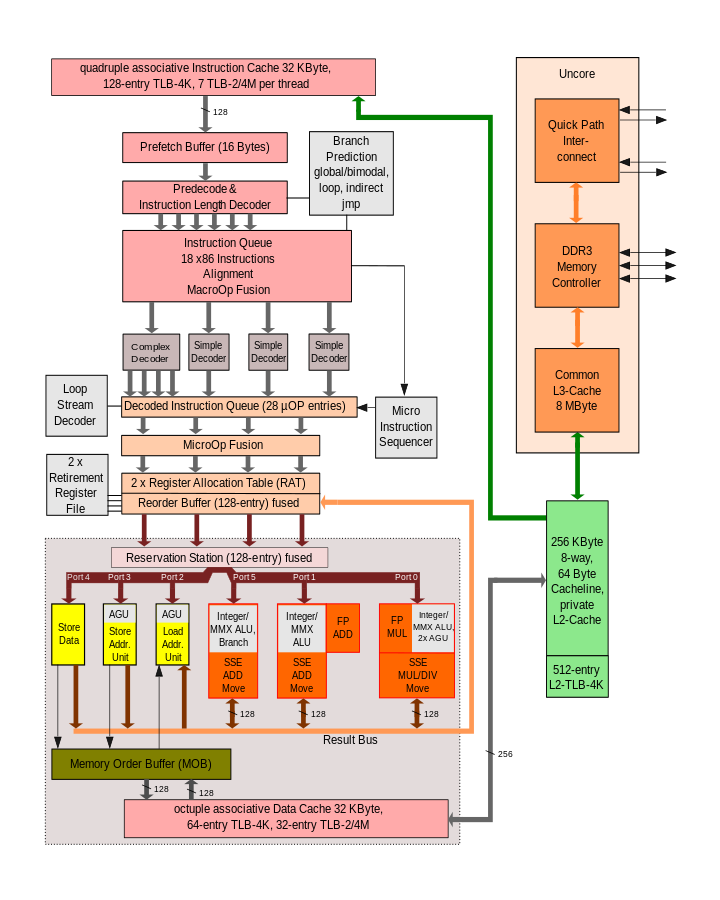
\includegraphics[height = .8\textheight]{Intel_Nehalem_arch}
%     \caption{Микроархитектура Intel Nehalem в 4-х ядерной реализации}
%   \end{figure}

%   \note{

%     На слайде представлено более полное описание микроархитектуры, но мы же
%     \textbf{рассмотрим упрощённую версию}.

%   }
% \end{frame}

\begin{frame}<1>[label = reorder_exe]{\insertsubsubsection. Не по порядку}

  \begin{figure}[h]
    \begin{tikzpicture}[
      align = center,
      ->,
      > = Stealth,
      thick,
      node distance = .6,
      block/.style = {
        rectangle,
        draw,
        fill = ForestGreen,
        text = White,
      },
      ]

      \node[block] (l1_i) {
        L1 I\$
      };

      \node[block, below = .3 of l1_i,
      rectangle split,
      rectangle split parts = 2] (if_id) {
        Instruction Fetch
        \nodepart{two}
        Instruction Decode
      };

      \node[block, left = 1 of if_id] (bp) {
        Branch \\
        Predictor
      };

      \node[block, below = of if_id] (rob) {
        Register Renaming (ROB)
      };

      \node[block, below left = of rob.south] (iprf) {
        Integer Physical \\
        Register File
      };

      \node[block, below right = of rob.south] (vprf) {
        Vector Physical \\
        Register File
      };

      \node[block, below = 2cm of rob] (eu) {
        Execution Units
      };

      \node[block, below = of eu] (l1_d) {
        L1 D\$
      };

      \node[block,
      minimum height = 4cm,
      minimum width = 1cm,
      right = 1cm of rob] (l2) {
        L2
      };

      \node<2>[
      fit = (bp),
      line width = 0.5mm,
      draw = red,
      ] (fit_bp) {};

      \node<2>[
      fit = (rob),
      line width = 0.5mm,
      draw = red,
      ] (fit_rob) {};

      \path (l1_i)  edge      (if_id)
            (if_id) edge[<->] (bp)
            (rob)   edge[<->] (iprf.north)
            (rob)   edge[<->] (vprf.north)
            (iprf)  edge[<->] (eu)
            (vprf)  edge[<->] (eu)
            (eu)    edge[<->] (l1_d);

      \foreach \i [count = \xi from 0] in {2,...,-2}{
        \draw ([xshift = \i * 0.4cm]if_id.south) -- ([xshift = \i * 0.4cm]rob.north);
      }

      \draw[<->] (l1_i) -| (l2.north);
      \draw[<->] (l1_d) -| (l2.south);

    \end{tikzpicture}
    \caption{Элементы системы выполнения современного процессора (выполнение
      инструкций не по порядку)}\label{fig:exe_out_of_order}
  \end{figure}

  \note<1>{

    Рисунок \ref{fig:exe_out_of_order}, \textbf{выполнение инструкций не по
      порядку}.

    Инструкции получаются и декодируются по порядку во \textbf{front-end}.

    \textbf{ROB} --- \textbf{Re-Order Buffer}.

    Именно поэтому процессор может выполнять несколько инструкций
    \textbf{одновременно}, при этом не обязательно в порядке их следования.
    Современные процессоры также могут параллельно выполнять одни и те же стадии
    для оптимизации вычислений.

  }

  \note<2->{

    О работе Reorder Buffer \textbf{рассказано не будет}, существует множество
    его реализаций.

    Ниже \textbf{будет рассказано} о работе этих элементов.

  }
\end{frame}

% \begin{frame}{\insertsubsubsection. Не по порядку}

%   \begin{figure}[h]
%     \begin{tikzpicture}[
%       align = center,
%       ->,
%       > = Stealth,
%       thick,
%       double = ForestGreen,
%       double distance = 1pt,
%       % node distance = .6,
%       c_node/.style = {
%         circle,
%         draw,
%         fill = ForestGreen,
%         text = White,
%         minimum width = 1cm,
%         text width = .5cm,
%         text centered,
%       },
%       block/.style = {
%         rectangle,
%         draw,
%         fill = ForestGreen,
%         text = White,
%         minimum width = 3cm,
%         text width = 3cm,
%         text centered,
%       },
%       ]

%       \node[block,
%       rectangle split,
%       rectangle split parts = 6] (code) {
%         R1 = LOAD A \\
%         \nodepart{two}
%         R2 = LOAD B \\
%         \nodepart{three}
%         R3 = R1 + R2 \\
%         \nodepart{four}
%         R1 = 1 \\
%         \nodepart{five}
%         R2 = 2 \\
%         \nodepart{six}
%         R3 = R1 + R2 \\
%       };

%       \node[c_node, right = 3 of code.north east] (r1_1) {
%         R1
%       };

%       \node[c_node, right = of r1_1] (r2_1) {
%         R2
%       };

%       \node[c_node, below = of $(r1_1)!0.5!(r2_1)$,
%       label = right:Есть зависимость от данных] (r3_1) {
%         R3
%       };

%       \node[c_node, below = 2 of r1_1] (r1_2) {
%         R1
%       };

%       \node[c_node, right = of r1_2] (r2_2) {
%         R2
%       };

%       \node[c_node, below = of $(r1_2)!0.5!(r2_2)$,
%       label = right:Нет зависимости от данных] (r3_2) {
%         R3
%       };

%       \path (r1_1) edge (r3_1)
%       (r2_1) edge (r3_1)
%       (r1_2) edge (r3_2)
%       (r2_2) edge (r3_2);

%     \end{tikzpicture}
%     \caption{Пример выполнения инструкций не по
%       порядку}\label{fig:exe_out_of_order_example}
%   \end{figure}

%   \note{

%     Представлен пример кода, который имеет и зависимые, и независимые от других
%     данных участки. \textbf{На следующем слайде} будет представлено, как RoB
%     обрабатывает такой код.

%   }
% \end{frame}

% \begin{frame}{\insertsubsubsection. Не по порядку}

%   \begin{columns}
%     \begin{column}{.3\textwidth}
%       \begin{figure}[h]
%         \center
%         \begin{tikzpicture}[
%           align = center,
%           thick,
%           block/.style = {
%             rectangle,
%             draw,
%             text = White,
%             minimum width = 3cm,
%             text width = 3cm,
%             text centered,
%           },
%           ]

%           \node[block,
%           rectangle split,
%           rectangle split parts = 6,
%           rectangle split part fill = {Maroon, Maroon, Maroon, ForestGreen, ForestGreen, ForestGreen},
%           ] (code) {
%             R1 = LOAD A \\
%             \nodepart{two}
%             R2 = LOAD B \\
%             \nodepart{three}
%             R3 = R1 + R2 \\
%             \nodepart{four}
%             R1 = 1 \\
%             \nodepart{five}
%             R1 = 2 \\
%             \nodepart{six}
%             R3 = R1 + R2 \\
%           };
%         \end{tikzpicture}
%         \caption{Порядок выполнения}
%       \end{figure}
%     \end{column}

%     \begin{tikzpicture}
%       \draw[line width = 3pt, -{Stealth[length = 1cm]}] (-2,0) -- (0,0);
%     \end{tikzpicture}

%     \begin{column}{.6\textwidth}
%       \begin{table}[h]
%         \begin{tabular}{|c|m{1.4cm}|c|m{1.3cm}|m{1cm}|}
%           \hline
%           №&Имя регистра&Инструкция&Зависи\-мости&Гото\-во?\\
%           \hline%
%           \rowcolor{Maroon}%
%           \color{White}1&\color{White}P1 = R1&\color{White}P1 = LOAD A&\color{White}-&\color{White}-\\
%           \hline%
%           \rowcolor{Maroon}%
%           \color{White}2&\color{White}P2 = R2&\color{White}P2 = LOAD B&\color{White}-&\color{White}-\\
%           \hline%
%           \rowcolor{Maroon}%
%           \color{White}3&\color{White}P3 = R3&\color{White} P3 = P1 + P2&\color{White} 1, 2&\color{White}-\\
%           \hline%
%           \rowcolor{ForestGreen}%
%           \color{White}4&\color{White}P4 = R1&\color{White}P4 = 1&\color{White}-&\color{White}+\\
%           \hline%
%           \rowcolor{ForestGreen}%
%           \color{White}5&\color{White}P5 = R2&\color{White}P5 = 1&\color{White}-&\color{White}+\\
%           \hline%
%           \rowcolor{ForestGreen}%
%           \color{White}6&\color{White}P6 = R3&\color{White}P6 = P4 + P5&\color{White}4, 5&\color{White}-\\
%           \hline%
%         \end{tabular}
%         \caption{Re-Order Buffer (ROB)}
%       \end{table}
%     \end{column}
%   \end{columns}

%   \note{

%     RoB \textbf{внутри себя производит трансляцию} в требуемый ему вид,
%     переименовывает регистры, реорганизует опкоды.

%     Именно по этой причине код может исполняться внутри процессора не по
%     порядку.

%   }

% \end{frame}

\againframe<2>{reorder_exe}

\subsubsection{Оптимизатор потока инструкций}
\begin{frame}{\insertsubsubsection}


  \begin{figure}[h]
    \begin{tikzpicture}[
      align = center,
      ->,
      > = Stealth,
      thick,
      double = ForestGreen,
      double distance = 1pt,
      % node distance = .6,
      block/.style = {
        rectangle,
        draw,
        fill = ForestGreen,
        text = White,
        minimum width = 4cm,
        text width = 4cm,
        text centered,
      },
      ]

      \node[block] (if) {
        \texttt{if x > y}
      };

      \node[block, below left = of if.center] (secret) {
        \texttt{get\_secret\_key()}
      };

      \node[block, below right = of if.center] (comp) {
        \texttt{some\_computation()}
      };

      \draw (if.west) -| node[above] {$\omega = 0.80$} (secret.north);
      \draw (if.east) -| node[above] {$\omega = 0.53$} (comp.north);

    \end{tikzpicture}
    \caption{\texttt{get\_secret\_key()} может выполниться
      спекулятивно}\label{fig:if_speculative_example}
  \end{figure}

  \note{

    Ещё одна идея для повышения производительности процессора ---
    \textbf{исполнение инструкций спекулятивно}. С помощью такой оптимизации
    процессор \textbf{угадывает возможный переход и исполняет его} прежде, чем
    он может выполниться на самом деле. Если угаданный путь был верным, то
    процессор просто берёт информацию, которую получил заранее, в противном
    случае \textbf{информация} о ходе спекулятивного выполнения просто
    \textbf{удаляется}.

    Существуют:

    \begin{itemize}
    \item Статическое предсказание
    \item Динамическое предсказание
      \begin{itemize}
      \item счётчик с насыщением
      \item адаптивный двухуровневый предсказатель
      \item локальный предсказатель перехода
      \item глобальный предсказатель перехода
      \item гибридный предсказатель перехода
      \item предсказатель для цикла
      \item предсказатель косвенных переходов
      \item предсказатель инструкций возврата
      \item предсказатель, основанный на машинном обучении
      \end{itemize}
    \end{itemize}

  }
\end{frame}

\subsubsection{Многоядерность}
\begin{frame}{\insertsubsubsection}

  \begin{figure}[h]
    \center%
    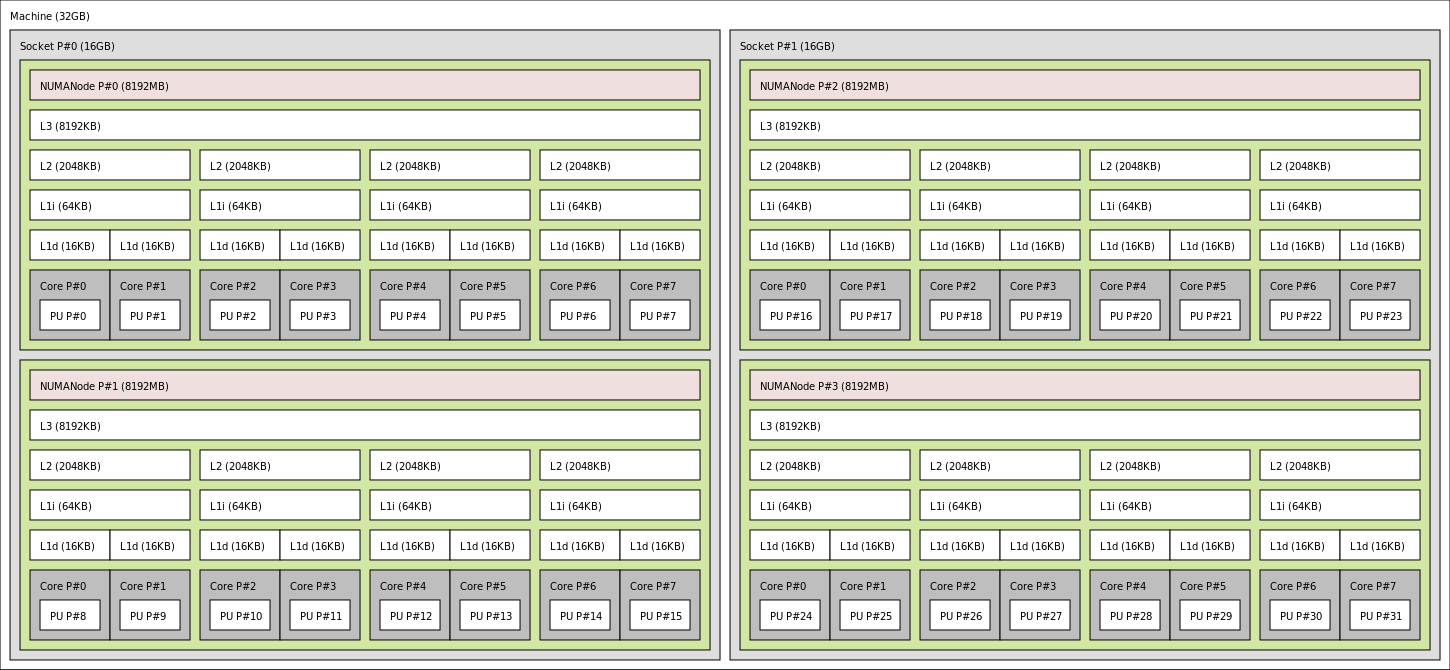
\includegraphics[height = .8\textheight]{Hwloc}
    \caption{Архитектура многоядерного процессора AMD Bulldozer}
  \end{figure}

  \note{

    Вместо оптимизации скорости выполнения на единственном ядре, также
    существует возможность \textbf{увеличивать количество этих самых ядер}.
    Особенно часто много ядер установлено в процессорах, работающих на серверах,
    это позволяет выполнять многие независимые друг от друга задачи параллельно.
    Однако, если задачу невозможно распараллелить, то прироста в
    производительности, конечно же, не будет. В настоящее время, \textbf{почти
      любое устройство имеет несколько ядер}, в том числе IoT устройства и
    домашние компьютеры. К тому же, многие языки программирования позволяют без
    лишних сложностей писать приложения, которые будут исполнятся на нескольких
    ядрах. \textbf{Каждое} из таких \textbf{ядер имеет свои приватные ресурсы},
    например, регистры и конвейеры выполнения, а также \textbf{общие ресурсы},
    например, основной доступ к памяти.

  }
\end{frame}
